% debut d'un fichier latex standard
\documentclass[a4paper,12pt,twoside]{article}

\usepackage{lipsum}
\usepackage{empheq}

% pour l'inclusion de figures en eps,pdf,jpg
\usepackage{graphicx}
\usepackage{subcaption}
\usepackage{wrapfig}
% quelques symboles mathematiques en plus
\usepackage{amsmath}
\usepackage{amsthm} % Pour les preuves
% le tout en langue francaise
%\usepackage[french]{babel}
% on peut ecrire directement les caracteres avec l'accent
% a utiliser sur Linux/Windows
\usepackage[utf8]{inputenc}
\usepackage[T1]{fontenc}
% a utiliser sur le Mac
%\usepackage[applemac]{inputenc}
% pour l'inclusion de links dans le document
\usepackage[colorlinks,bookmarks=false,linkcolor=blue,urlcolor=blue]{hyperref}
\usepackage{siunitx}
% pour les degrés
\usepackage{textcomp}
\paperheight=297mm
\paperwidth=210mm

\setlength{\textheight}{235mm}
\setlength{\topmargin}{-1.2cm} % pour centrer la page verticalement
%\setlength{\footskip}{5mm}
\setlength{\textwidth}{15cm}
\setlength{\oddsidemargin}{0.56cm}
\setlength{\evensidemargin}{0.56cm}

\pagestyle{plain}

% quelques abreviations utiles
\def \be {\begin{equation}}
\def \ee {\end{equation}}
\def \dd  {{\rm d}}

\newcommand{\mail}[1]{{\href{mailto:#1}{#1}}}
\newcommand{\ftplink}[1]{{\href{ftp://#1}{#1}}}

\newcommand{\illabel}[1]{ ~ \refstepcounter{equation}(\theequation)\label{#1}} % Ecrit une équation dans le texte, numérotés.
\newcommand{\mbf}[1]{\mathbf{#1}} % bold font in math
\newcommand{\grad}[1]{\nabla#1}
\newcommand{\Div}[1]{\nabla\cdot\mathbf{#1}}
\newcommand{\rot}[1]{\nable\cross\mathbf{#1}}
\newcommand{\bracket}[1]{\left(#1\right)}
\newcommand{\sqbracket}[1]{\left[#1\right]}
\newcommand{\lapl}[1]{\Delta#1}

%
% latex SqueletteRapport.tex      % compile la source LaTeX
% xdvi SqueletteRapport.dvi &     % visualise le resultat
% dvips -t a4 -o SqueletteRapport.ps SqueletteRapport % produit un PostScript
% ps2pdf SqueletteRapport.ps      % convertit en pdf

% pdflatex SqueletteRapport.pdf    % compile et produit un pdf
% \message{================> TAILLE DE LA POLICE EN CM \printinunitsof{cm}\prntlen{\textwidth}}

% ======= Le document commence ici ======

\begin{document}
% Le titre, l'auteur et la date
\title{Electrostatics\\{\small Physique Numérique I}\\{\small Rapport 6}}
\date{\today}
\author{Delphine Martres et Damien Korber\\{\small \mail{delphine.martres@epfl.ch} et \mail{damien.korber@epfl.ch}}}

\maketitle
\tableofcontents % Table des matieres


% Quelques options pour les espacements entre lignes, l'identation
% des nouveaux paragraphes, et l'espacement entre paragraphes
\baselineskip=16pt
\parindent=15pt
\parskip=5pt
\newpage

%%%% ON COMMENCE A ECRIRE D'ICI

%TODO dans tout le document je crois : unités !

\section{Introduction}
In this report, we consider a dielectric occupying a volume of space $\Omega$ with the potential on the boundary $\partial\Omega$ at $V_0$, variable dielectric constant $\epsilon_r(\mathbf{x})$ and free charges density $\rho_{lib}(\mathbf{x})$.

\section{Differential equation and variational form}
  \subsection{Differential equation for the potential $\phi(\vec{x})$} \label{sec:equa-diff-phi}
    This section will derive the equation that describes the problem.
    \begin{align*}
      \intertext{First, one of Maxwell's equations is used}
      \nabla\cdot\mathbf{D} &= \rho\bracket{\mathbf{x}} \\
      \intertext{where $\mathbf{D}=\epsilon_0\epsilon_r\mathbf{E}$ is the electric displacement field.}
      \nabla\cdot\bracket{\epsilon_0\epsilon_r\mathbf{E}} &= \rho\bracket{\mathbf{x}} \\
      \nabla\cdot\bracket{\epsilon_r\mathbf{E}} &= \frac{\rho\bracket{\mathbf{x}}}{\epsilon_0} \\
      \epsilon_r\Div{E} + \mathbf{E}\cdot\nabla\epsilon_r &= \frac{\rho\bracket{\mbf{x}}}{\epsilon_0} \\
      \intertext{We know that $\mbf{E}$ derive from a potential $\phi$ such that $\mathbf{E}=-\grad{\phi}$. Thus}
      -\epsilon_r\lapl{\phi}-\grad{\phi}\grad{\epsilon_r} &= \frac{\rho\bracket{\mbf{x}}}{\epsilon_0}
      \intertext{This leads to equation \eqref{eq:equa-diff}.}
    \end{align*}
    \begin{equation}
      \centering
      \boxed{\grad{\phi}\grad{\epsilon_r} + \epsilon_r\lapl{\phi} = -\frac{\rho\bracket{\mbf{x}}}{\epsilon_0}}
      \label{eq:equa-diff}
    \end{equation}

    with $\phi\bracket{\mbf{x}}=V_0~\forall\mbf{x}\in\partial\Omega$.

  \subsection{Variational form}
    To numerically solve equation \eqref{eq:equa-diff}, the variational form of the problem must be found.

    \begin{align*}
      \intertext{Let $\eta\bracket{\mbf{x}}\subset\mathcal{C}^1\bracket{\Omega}$, $\eta\bracket{\mbf{x}}=0~ \forall \mbf{x}\in\partial\Omega$. Multiply both sides of equation \eqref{eq:equa-diff} by $\eta\bracket{\mbf{x}}$, and integrate over the volume $\Omega$.}
      \int_\Omega \eta\bracket{\mbf{x}}\grad{\phi}\grad{\epsilon_r}d\mbf{x} + \int_\Omega \eta\bracket{\mbf{x}}\epsilon_r\lapl{\phi}d\mbf{x} &= -\int_\Omega \eta\bracket{\mbf{x}}\frac{\rho\bracket{\mbf{x}}}{\epsilon_0}d\mbf{x}
      \intertext{By using formula $\nabla\cdot\bracket{f\nabla g} = \grad{f}\cdot\grad{g} + f\lapl{g}$ where $f=\eta\epsilon_r$ et $g=\phi$:}
      \nabla\cdot\bracket{\eta\epsilon_r\grad{\phi}} &= \grad{\bracket{\eta\epsilon_r}}\cdot\grad{\phi} + \eta\epsilon_r\lapl{\phi} \\
      &= \epsilon_r\grad{\eta}\cdot\grad{\phi} + \eta\grad{\epsilon_r}\cdot\grad{\phi} + \eta\epsilon_r\lapl{\phi} \\
      \Rightarrow \int_\Omega\bracket{\eta\bracket{\mbf{x}}\grad{\phi}\cdot\grad{\epsilon_r} + \eta\bracket{\mbf{x}}\epsilon_r\lapl{\phi}}d\mbf{x} &= \int_\Omega\bracket{\underbrace{\nabla\cdot\bracket{\eta\epsilon_r\grad{\phi}}}_* - \epsilon_r\grad{\eta}\cdot\grad{\phi}}d\mbf{x}
      \intertext{Using Gauss' theorem: $*= \int_{\partial\Omega}\eta\epsilon_r\grad{\phi}\cdot d\mbf{\sigma} = 0$ because $\eta\bracket{\mbf{x}}=0~\forall\mbf{x}\in\partial\Omega$ by definition.}
    \end{align*}
    \begin{equation}
      \centering
      \boxed{\int_\Omega\epsilon_r\grad{\eta}\cdot\grad{\phi}d\mbf{x} = \int_\Omega\eta\bracket{\mbf{x}}\frac{\rho\bracket{\mbf{x}}}{\epsilon_0}d\mbf{x}}
      \label{eq:variational-form}
    \end{equation}

    with $\phi\bracket{\mbf{x}}=V_0~\forall\mbf{x}\in\partial\Omega$.

  \subsection{Special case: cylinder} %TODO : Faut changer le titre, il pue.
    From now, the exercice will focus on a cylinder of radius $R$ and of length $L_z$ long enough to neglect the side-effects.
    Thus, $\phi\bracket{r}$, $\epsilon_r\bracket{r}$ and $\rho_\text{lib}\bracket{r}$ only depend on the radius of the cylinder, so $\grad{\eta}=\frac{d\eta}{dr}$ and $\grad{\phi}=\frac{d\phi}{dr}$.
    From equation \eqref{eq:variational-form}, the variational form of the problem can be expressed in cylindrical coordinates, which gives equation \eqref{eq:variational-form-cylindrical}.

    \begin{equation}
      \centering
      \boxed{\int_0^R r\epsilon_r\bracket{r}\frac{d\eta\bracket{r}}{dr}\frac{d\phi\bracket{r}}{dr}dr = \frac{1}{\epsilon_0}\int_0^R r\eta\bracket{r}\rho\bracket{r} dr}
      \label{eq:variational-form-cylindrical}
    \end{equation}

    with $\phi\bracket{R} = V_0$.

    Note that $r$ is added to the integral, coming from the change of variable into cylindrical coordinates.

\section{Finite elements}
  The problem need to be discretized to get a numerical solution, so $\phi$ and $\eta$ must be expressed in a discretized way.
  Consider $\Lambda_i\bracket{r}$, the polynomials as represented on figure \ref{fig:lambda}.
  These function are used to approximate $\phi$ and $\eta$, which are given by equation \eqref{eq:approx-phi-eta}.

  \begin{equation}
    \phi\bracket{r}=\sum_j\phi_j\Lambda_j\bracket{r}~\text{and}~\eta\bracket{r}=\sum_i\eta_i\Lambda_i\bracket{r}
    \label{eq:approx-phi-eta} %TODO : Vérifier les indices. (être cohérent avec la suite surtout)
  \end{equation}

  \begin{figure}[h]
    \centering
    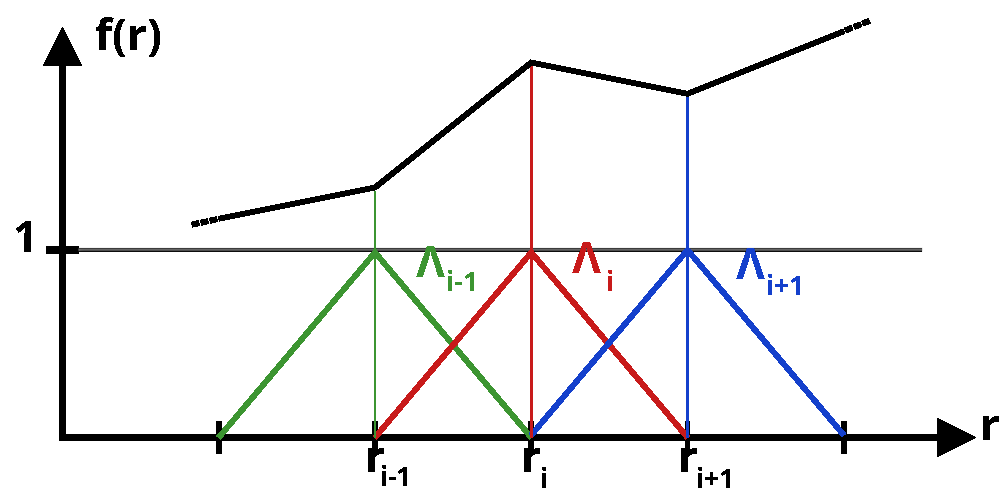
\includegraphics[width=0.6\textwidth]{graphs/lambda.pdf}
    \caption{Scheme of the lambda functions}
    \label{fig:lambda}
  \end{figure}

  Using equations \eqref{eq:variational-form-cylindrical} and \eqref{eq:approx-phi-eta}, the problem can be discretized as equation \eqref{eq:discret-gen}.

  \begin{equation}
    \sum_i\eta_i\sum_j\bracket{\int_0^R r\epsilon_r\frac{d\Lambda_i}{dr}\frac{d\Lambda_j}{dr}dr}\phi_j = \sum_i\eta_i\bracket{\int_0^R\Lambda_i\frac{\rho}{\epsilon_0}dr}
    \label{eq:discret-gen}
  \end{equation}

  By identification, a system of linear equation $A\mbf{\phi}=\mbf{b}$ can be deduced, as given by equation \eqref{eq:discret-final}.

  \begin{equation}
    \sum_j\bracket{\underbrace{\int_0^R r\epsilon_r\frac{d\Lambda_i}{dr}\frac{d\Lambda_j}{dr}dr}_{A_{ij}}}\phi_j = \underbrace{\int_0^R \Lambda_i\frac{\rho}{\epsilon_0}dr}_{b_i}
    \label{eq:discret-final}
  \end{equation}



  \subsection{Writing matrix $A$ and vector $\mbf{b}$ of the linear system $A\mbf{\phi}=\mbf{b}$}\label{sec:writing-A-b1} %TODO : Changer le titre, celui-là pue.

  For both computations, the trapezoidal rule will be needed:
  \begin{equation}
    \int_a^b f\bracket{x}dx = \bracket{b-a}\frac{f\bracket{b} + f\bracket{a}}{2}
    \label{eq:trapezoidal-rule}
  \end{equation}

  First, the matrix $A$ needs to be explicited.

  \begin{equation*}
   A_{ij} = \int_0^R r\epsilon_r(r)\frac{d\Lambda_i}{dr}\frac{d\Lambda_j}{dr}dr = \sum_{k=1}^N \int_{r_{k}}^{r_{k+1}}r \epsilon_r(r)\frac{d\Lambda_i}{dr}\frac{d\Lambda_j}{dr}dr
  \end{equation*}

  Since:
  \begin{equation}
   \frac{d\Lambda_i}{dr}= \begin{cases}
   \frac{1}{h_{i-1}} \text{ over } [r_{i-1},r_i]\\
   -\frac{1}{h_{i}} \text{ over } [r_i,r_{i+1}]\\
   0 \text{ elsewhere}
                          \end{cases}
    \label{eq:lambderiv}
  \end{equation}the last term is non-zero only if $i=j$ or $i=j+1$ or $i=j-1$. Three different cases thus have to be computed: $A_{ii}$ the terms on the diagonal, $A_{i,i+1}$ and $A_{i+1,i}$, respectively under and over the diagonal. Using equation \eqref{eq:trapezoidal-rule} we get equation \eqref{eq:A-final}

  \begin{align*}
   A_{ii} &= \int_{r_{i-1}}^{r_i} r\epsilon_r(r) \frac{1}{h_{i-1}^2} dr + \int_{r_i}^{r_{i+1}} r\epsilon_r(r) \frac{1}{h_i^2} dr\\
   &= \frac{1}{2 h_{i-1}} [r_i \epsilon_r(r_i)+r_{i-1}\epsilon_r(r_{i-1})] + \frac{1}{2 h_i} [r_i \epsilon_r(r_i)+r_{i+1}\epsilon_r(r_{i+1})]\\
  \end{align*}
  and
  \begin{align*}
   A_{i+1,i} = A_{i,i+1} &= \int_{r_i}^{r_{i+1}} r\epsilon_r(r) \frac{-1}{h_i^2} dr\\
   &= -\frac{1}{2 h_i} [r_i \epsilon_r(r_i)+r_{i+1}\epsilon_r(r_{i+1})]\\
  \end{align*}

  \begin{empheq}[box=\boxed]{align}
    \begin{split}
      A_{ii} &= \frac{1}{2 h_{i-1}} [r_i \epsilon_r(r_i)+r_{i-1}\epsilon_r(r_{i-1})] + \frac{1}{2 h_i} [r_i \epsilon_r(r_i)+r_{i+1}\epsilon_r(r_{i+1})]\\
      A_{i+1,i} = A_{i,i+1} &= -\frac{1}{2 h_i} [r_i \epsilon_r(r_i)+r_{i+1}\epsilon_r(r_{i+1})]\\
    \end{split}
    \label{eq:A-final}
  \end{empheq}

  Now, vector $\mbf{b}$ needs to be explicited.

  \begin{align*}
    b_i &= \int_0^R r\Lambda_i\frac{\rho\bracket{r}}{\epsilon_0}dr = \sum_{k=1}^N \int_{r_{k}}^{r_{k+1}}r\Lambda_i\frac{\rho\bracket{r}}{\epsilon_0}dr
    \intertext{Knowing that $\Lambda_i\bracket{r_k} = \delta_{ik}$ and using the trapezoidal rule (Eq. \eqref{eq:trapezoidal-rule}):}
    &= \sum_{k=1}^N \frac{h_k}{2}\bracket{r_{k+1}\Lambda_i\bracket{r_{k+1}}\frac{\rho\bracket{r_{k+1}}}{\epsilon_0} + r_k\Lambda_i\bracket{r_k}\frac{\rho\bracket{r_k}}{\epsilon_0}} \\
    &= \frac{h_{i-1}}{2}r_i\frac{\rho\bracket{r_i}}{\epsilon_0} + \frac{h_i}{2}r_i\frac{\rho\bracket{r_i}}{\epsilon_0} = \frac{r_i\rho\bracket{r_i}}{2\epsilon_0}\bracket{h_{i-1} + h_i}
  \end{align*}

  \begin{equation}
    \boxed{b_i = \frac{r_i\rho\bracket{r_i}}{2\epsilon_0}\bracket{h_{i-1} + h_i}}
    \label{eq:b-final}
  \end{equation}

  Note that equation \eqref{eq:A-final} and \eqref{eq:b-final} are not the one implemented in the c++ source file.
  Instead of directly implementing the trapezoidal rule, a better approximation for this integral has been used: the trapezoidal-middle point rule.
  However, this approximation is fully compatible with the trapezoidal rule, as taking parameter $p=1$ gives the trapezoidal rule.
  See section \ref{sec:trapezoidal-middle-rule} for further informations. %TODO : paragraphe ajouté -D

  \section{Trivial case}

  In this section the parameters are $b=0.06$ m, $R=0.12$ m and $N_1=N_2$. The trivial case $\rho_{lib}(r)=\epsilon_0$ and $\epsilon_r(r)=1$ is studied to test the algorithm.

  \subsection{Comparison of numerical and analytical results}

  \begin{figure}[h!]
   \centering
   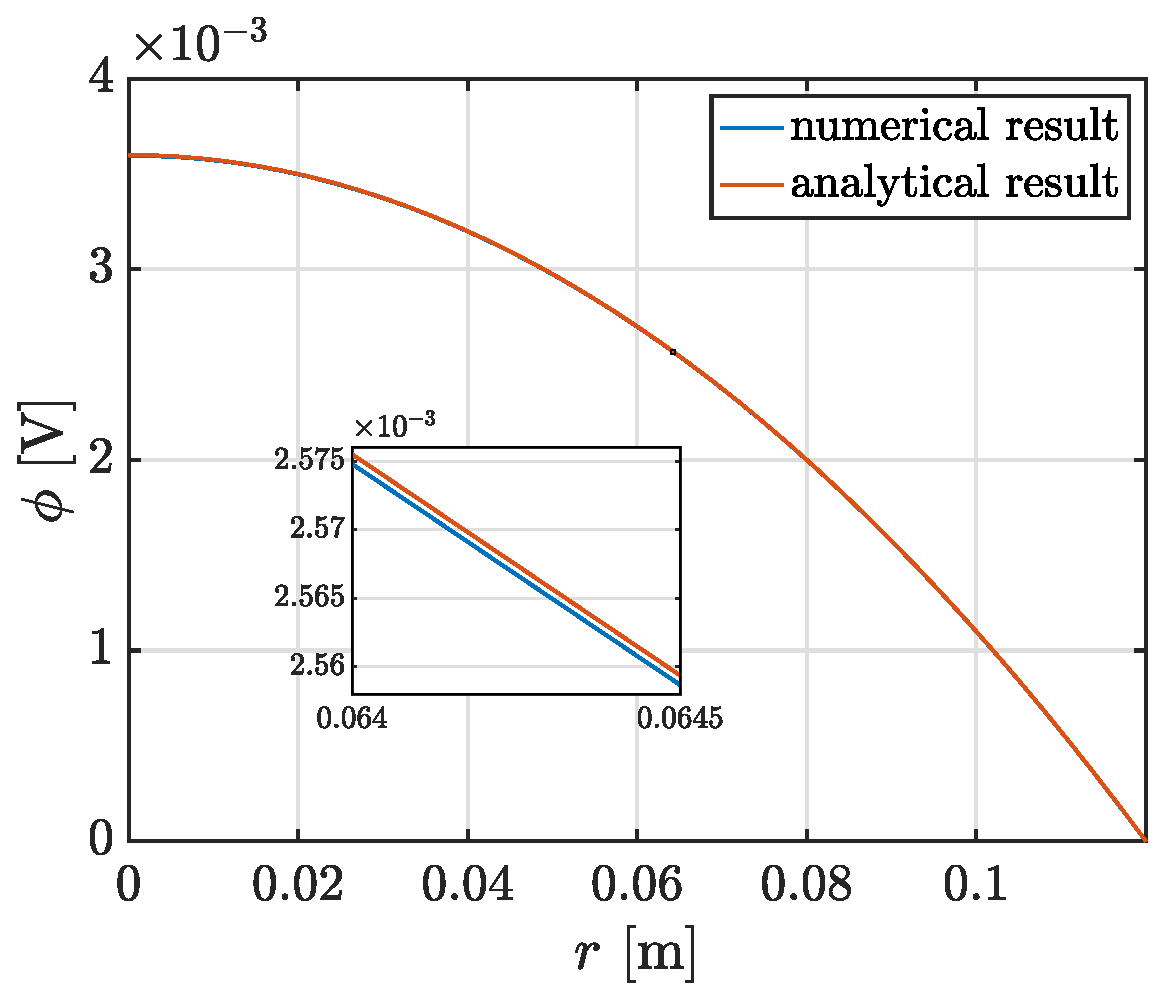
\includegraphics[width=0.5\textwidth]{graphs/c_phi.eps}
   \caption{Numerical and analytical potential in function of radius for N=20}
   \label{cphi}
  \end{figure}

  In fig. \ref{cphi}, the potential curve obtained with the algorithm is compared to the potential curve computed analytically: by applying the trivial case to eq.\eqref{eq:equa-diff} and using the boundary condition $\phi(R)=V_0=0$ V, we get the solution given by equation \eqref{phith}.
  \begin{equation}
   \phi(r)_{th} = \frac{R^2-r^2}{4} %TODO : Equation corrigée pour la rendre plus jolie. -D
   \label{phith}
  \end{equation}

  The difference between the curves is of order $10^{-6}$, and gets smaller as the radius increases, until the boundary of the cylinder, on which both curves reach the boundary condition of $\phi(R)=0$ V.

  \begin{figure}[h!]
   \centering
   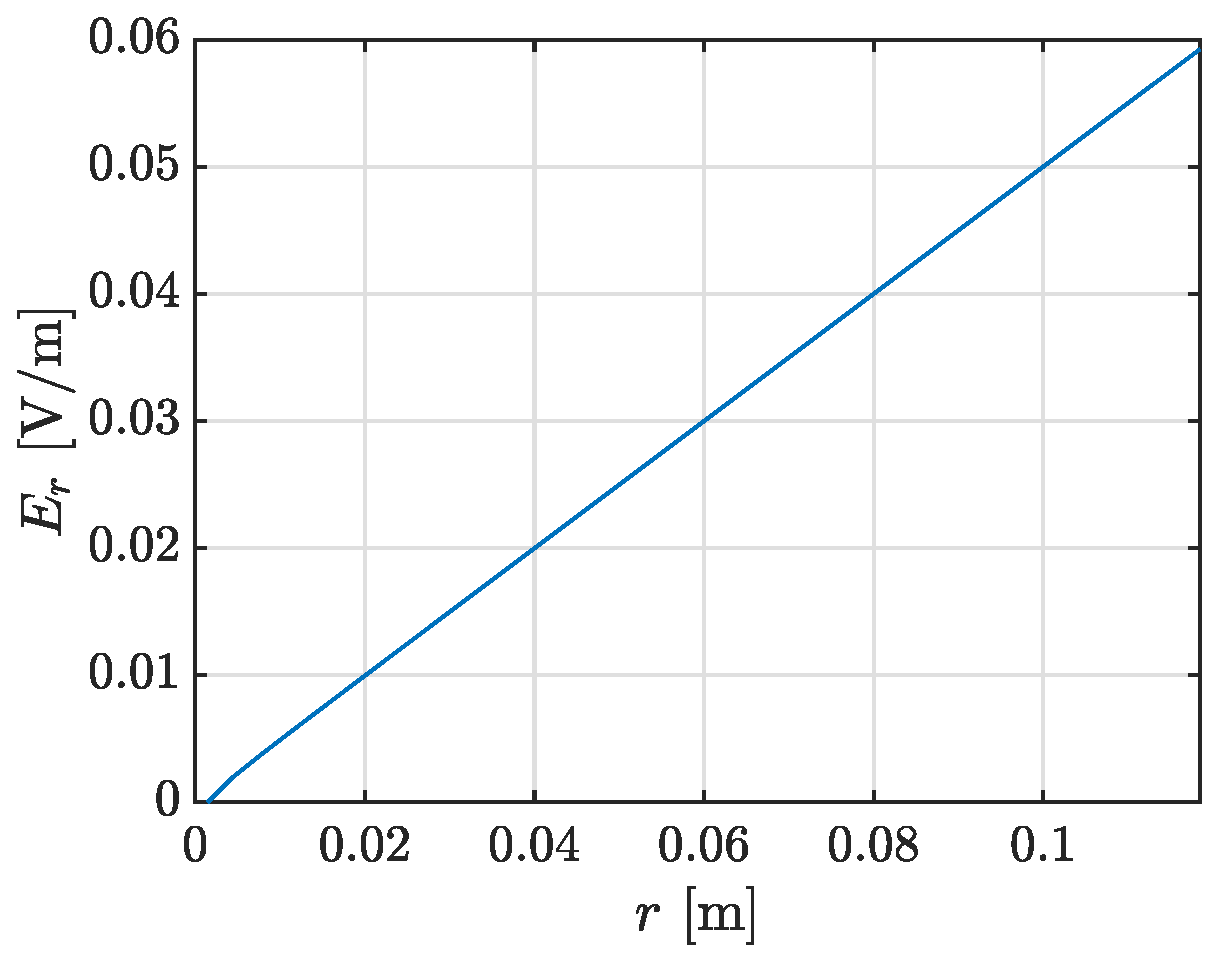
\includegraphics[width=0.5\textwidth]{graphs/c_Er.eps}
   \caption{Electric field in function of radius for N=20}
   \label{cEr}
  \end{figure}

  Fig. \ref{cEr} shows that the electric field is linear with respect to the radius of the cylinder.
  This is expected as $E_r = -\grad{\phi(r)} = -\frac{d\phi(r)}{dr}$, and $\phi(r)$ is quadratic.
  There is however an anomaly, as the curve should pass through the origin $(0,0)$, since the rate of variation of $\phi(r)$ around $r=0$ is null, however the first point is slighlty displaced to the right (at around $r=1.5\times 10^{-3}$).
  % This imprecision might come from a mistake in the matrix equation resolution algorithm, as the other groups had the same problem.
  This inaccuracy might come from the approximation made by using the trapezoidal rule, or by the discretization of the problem, as both are the only real source of error in this report.
  Note that some approximations are produced by the numerical rounding, but those are much smaller, so are neglected. %TODO : Phrase corrigée. -D

  \subsection{Convergence of $\phi(0)$}

  \begin{figure}[h]
   \centering
   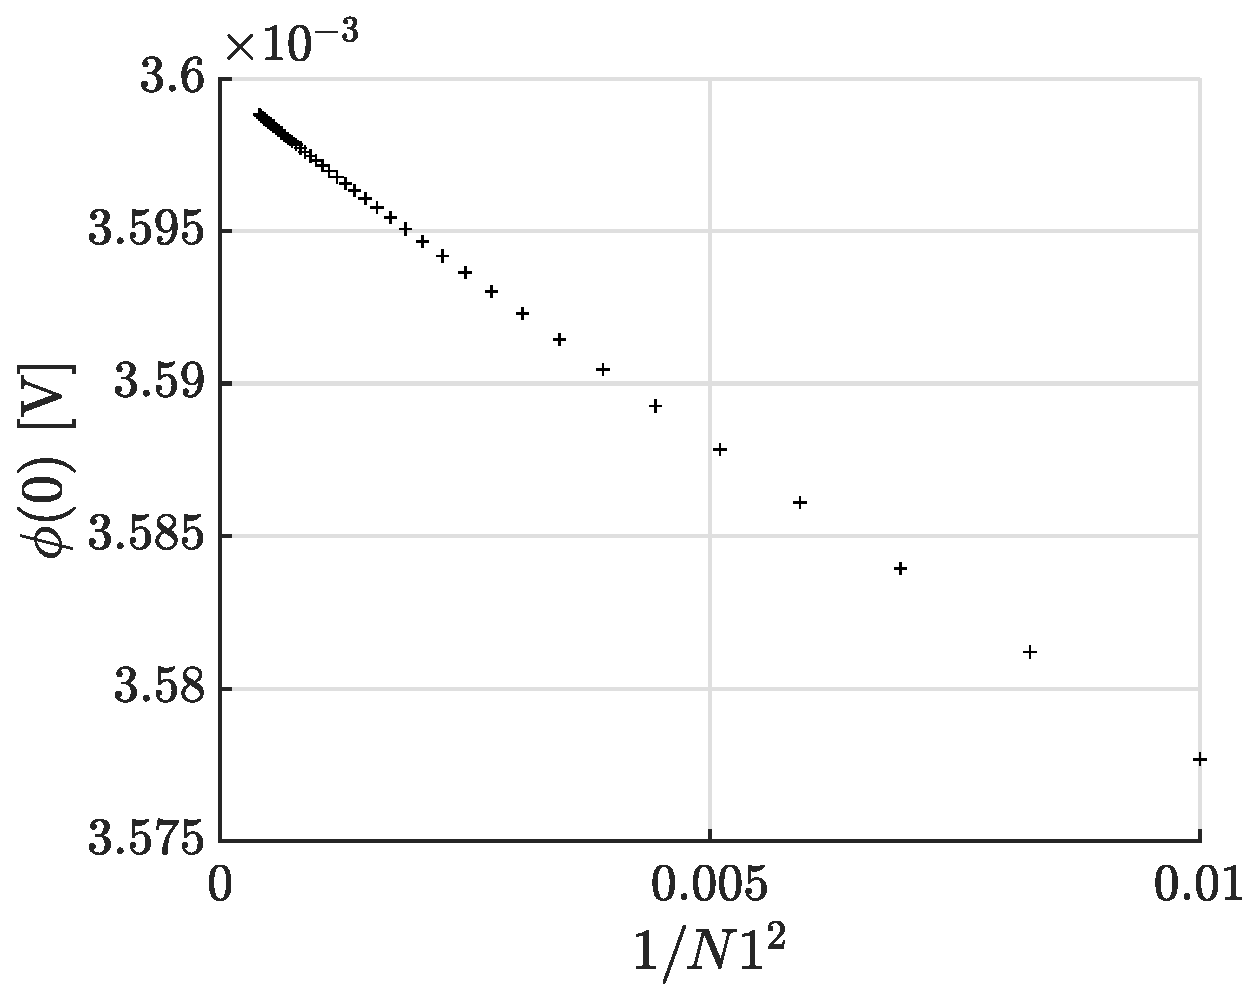
\includegraphics[width=0.6\textwidth]{graphs/c_convphi.eps}
   \caption{Convergence of the error on $\phi(0)$ with respect to $N1$}
   \label{cconv}
  \end{figure}

  On the log-log plot of fig. \ref{cconv}, we can see that the error $|\phi(0)-\phi(0)_{th}|$ on the numerical values of $\phi(0)$ converges with order $1.828$ with respect to $N1$.
  %TODO : Y'a rien à dire de plus ? -D

  \section{Non-trivial case}
  In this section, $b=\SI{0.02}{\m}$ and $R=\SI{0.12}{\m}$. Moreover, $\epsilon_r$ is given by equation \eqref{eq:def-er} and $\rho_{lib}$ is given by equation \eqref{eq:def-rholib}.

  \begin{align}
    \begin{split}
      \epsilon_r\bracket{r} := \begin{cases}
        1~&\text{if}~\bracket{0\leq r\leq b},\\
        8-6\frac{r-b}{R-b}~&\text{if}~\bracket{b\leq r\leq R}.
      \end{cases}
    \end{split}
    \label{eq:def-er}
  \end{align}

  \begin{align}
    \begin{split}
      \rho_{lib}\bracket{r} := \begin{cases}
        \epsilon_0 a_0\bracket{1-\bracket{\frac{r}{b}}^2}~&\text{if}~\bracket{0\leq r\leq b},\\
        0~&\text{if}~\bracket{b\leq r\leq R}.
      \end{cases}
    \end{split}
    \label{eq:def-rholib}
  \end{align}

  with $a_0=\SI{d4}{\volt\per\square\meter}$.

  Furthermore, the number of nodes on the horizontal axis and the vertical axis are linked by the relation: $N_2 = 2N_1$.
  Note that on this section, the trapezoidal rule has been used for evaluating the integrals. $\bracket{p=1\text{, see section \ref{sec:trapezoidal-middle-rule}}}$.


  \subsection{Comparison of different numerical solutions for $\phi\bracket{r}$ and $E\bracket{r}$}
  This section focuses on the comparison of the solutions of $\phi\bracket{r}$ and $E\bracket{r}$ for different meshes.
  The result can be seen on figure \ref{fig:d1-evo}.

  The first part to analyse is the point $r=b$ which is special on both figure \ref{fig:d1-evoPhi} and \ref{fig:d1-evoEr}.
  On figure \ref{fig:d1-evoPhi}, the point seems to be continuous, but is not differentiable.
  This non-differentiability leads to a discontinuity of $E\bracket{r}$ on figure \ref{fig:d1-evoEr}, as both are linked by the gradient operator.
  This discontinuity comes from the fact the point represents the interface between the dielectric and the vacuum inside the cylinder (or another medium with $\epsilon_r=1$).
  Physically, vacuum does not inhibit the electric field, as no opposed electric field is present (supposing no external electric field).
  On the other hand, dielectrics contains polarization charges that are polarized when applied to an external electric field. \cite{wiki:dielectrics}
  This polarization leads to the establishment of an electric field, which opposes the external one.
  Thus, the resulting electric field in the dielectric is lower than in the vacuum.
  The fact is that the permittivity transition between the vacuum and the dielectric is not smooth, as $\lim_{r\rightarrow b^-}\epsilon_r\bracket{r} = 1 \neq 8 = \lim_{r\rightarrow b^+}\epsilon_r\bracket{r}$. Thus, the electric field is not smooth.\\ %TODO : Faut faire gaffe, "smooth" est un terme mathématique. -D

  Regarding the comparison between the meshes, the main point is that the difference between the four case is low regarding the precision.
  On both figures, a zoom is needed to really differentiate the cases.
  The first simulation ($N_1=10, N_2=20$) is the only one that slightly diverges from the others, as can be seen from the zoom in the plots.
  Thus, choosing a setting around ($N_1=40, N_2=80$) seems enough regarding the precision, as more does not significantly change the result.\\

  \begin{figure}[h]
    \centering
    \begin{subfigure}{0.45\textwidth}
      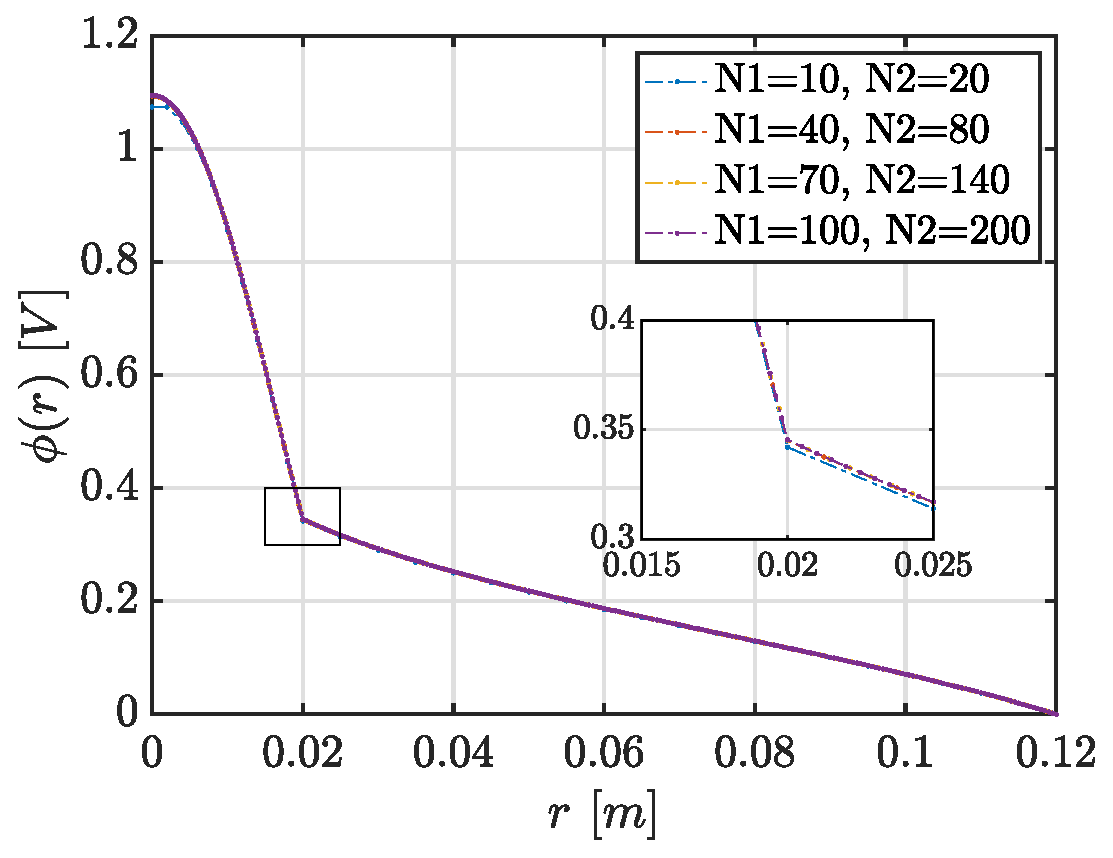
\includegraphics[width=\textwidth]{graphs/exd1-evoPhi}
      \caption{Evolution of $\phi\bracket{r}$}
      \label{fig:d1-evoPhi}
    \end{subfigure}
    ~
    \begin{subfigure}{0.45\textwidth}
      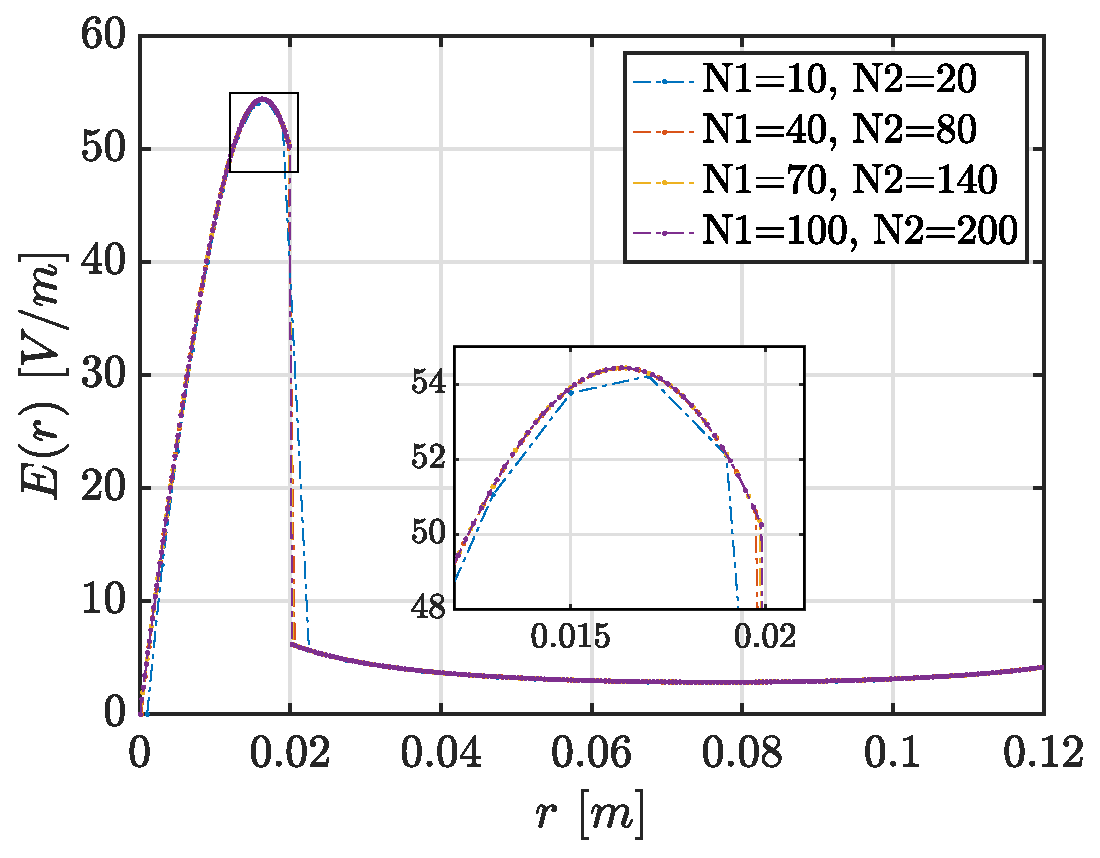
\includegraphics[width=\textwidth]{graphs/exd1-evoEr}
      \caption{Evolution of $E(r)$}
      \label{fig:d1-evoEr}
    \end{subfigure}
    \caption{Evolution of two quantities with respect to the distance $r$ from the center of the cylinder, for four simulations}
    \label{fig:d1-evo}
  \end{figure}

  \subsection{Convergence study of $\phi\bracket{r=b}$}
  This section focuses on the study of the convergence of $\phi\bracket{r}$ at $r=b$.
  Figure \ref{fig:d1-conv} gives the result of this experiment.
  The analytical solution for this problem could not be computed, so this figure does not study the error on the solution, but the convergence on a result.
  What can be seen is that $\phi\bracket{r}$ converges approximately to the 2nd order, as the plot is linear for a $1/N^2$ horizontal axis.

  \begin{figure}[h]
    \centering
    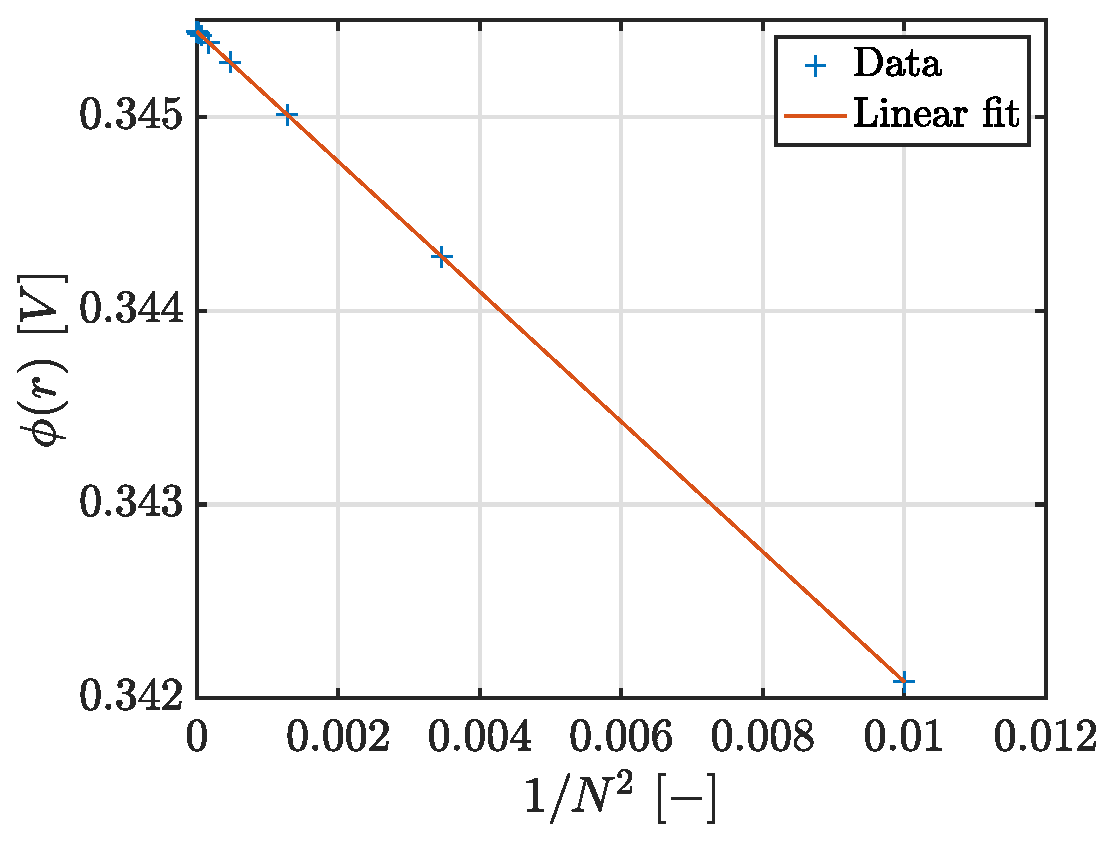
\includegraphics[width=0.5\textwidth]{graphs/exd1-convPhi.eps}
    \caption{Convergence of $\phi\bracket{r=b}$ for ten simulations. Note that $N=N_1$.}
    \label{fig:d1-conv}
  \end{figure}

  \subsection{Verification of $\Div{\mbf{D}\bracket{\mbf{x}}}$}
  This section focuses on the verification of a Maxwell's equation, $\Div{D}\bracket{\mbf{x}}$, using a finite difference method for the operator d/dr.
  The problem is in cylindrical coordinates, thus $\Div{D} = \frac{1}{r}\frac{d}{dr}\bracket{r\mbf{D}}$.
  Using the finite difference method, $\Div{D}$ is given by equation \eqref{eq:divDr-DF}.

  \begin{equation}
    \Div{D}\bracket{r_{\text{midmid},i}} = \frac{r_{\text{mid},i+1}\cdot D\bracket{r_\text{mid, i+1}} - r_{\text{mid},i}\cdot D\bracket{r_\text{mid, i}}}{r_{\text{mid},i+1} - r_{\text{mid},i}}\cdot\frac{1}{r_{\text{midmid},i}}
    \label{eq:divDr-DF}
  \end{equation}

  Figure \ref{fig:d2} gives the result for this computation.
  As can be seen, the quantities match exactly, which is the expected result.
  %TODO : T'as encore un truc à dire là dessus ? J'ai rien à dire. :|

  % Maxwell's law used at the beginning of section \ref{sec:equa-diff-establishment} states that the divergence of the displacement field is equal to the charge density.
  % However, this charge density considers every charges of the environment: free charges and polarization charges.

  \begin{figure}[h]
    \centering
    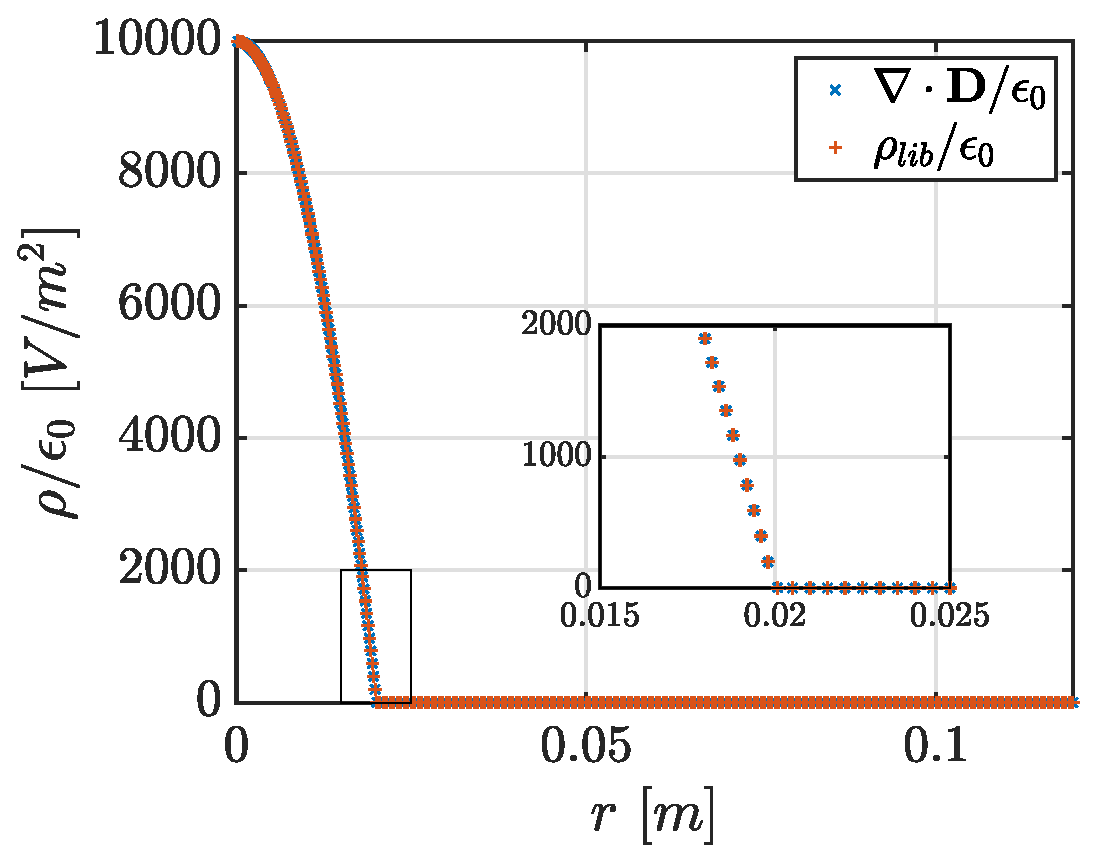
\includegraphics[width=0.5\textwidth]{graphs/exd2-diff.eps}
    \caption{Evolution of two quantities with respect to the distance $r$ from the center of the cylinder. Note that $N_2=2N_1=200$ for this simulation.} %TODO : La caption pue, non ?
    \label{fig:d2}
  \end{figure}

  \subsection{Computation of the polarization charge density $\rho_{pol}$} \label{sec:rhopol}
    The goal of this paragraph is to obtain the polarization charge density of the dielectrics.
    The polarization charges are the charges on the dielectrics that can not move, which forms a multitude of electrical dipoles. \cite{feynman:dielectrics}
    The density of polarization charges can be found using equations \eqref{eq:def-polarization} and \eqref{eq:def-rhopol}, coming from Feynman lectures on physics. \cite{feynman:dielectrics}

    \begin{align}
      \mbf{P} &= \mbf{D} - \epsilon_0\mbf{E}
      \label{eq:def-polarization} \\
      \rho_{pol} &= -\Div{\mbf{P}}
      \label{eq:def-rhopol}
    \end{align}

    where $\mbf{P}$ is the polarization.
    Thus, by combining them, equation \eqref{eq:rhopol-final} follows.

    \begin{align*}
      \rho_{pol} &= -\Div{\mbf{P}} = -\nabla\cdot\bracket{\mbf{D} - \epsilon_0\mbf{E}}\\
                 &= \epsilon_0\bracket{\Div{E} - \frac{\Div{D}}{\epsilon_0}}
    \end{align*}



    \begin{equation}
      \boxed{\frac{\rho_{pol}}{\epsilon_0} = \Div{E} - \frac{\Div{D}}{\epsilon_0}}
      \label{eq:rhopol-final}
    \end{equation}

    Using equation \eqref{eq:rhopol-final}, the evolution of the polarization charge density with respect to $r$ can be viewed on figure \ref{fig:rhopol}.
    The major information of this figure is the discontinuity point at $r=b$.
    This point tells that the overwhelming majority of the charges are located on the border of the dielectric.
    Note that, as $N_1$ and $N_2$ increase, the "discontinuity triangle" becomes thiner.
    This shows that the charges are not scattered around the border, but are located exactly on the interface between void and the dielectric.
    %TODO : Encore un truc à dire ?

    \begin{figure}[h]
      \centering
      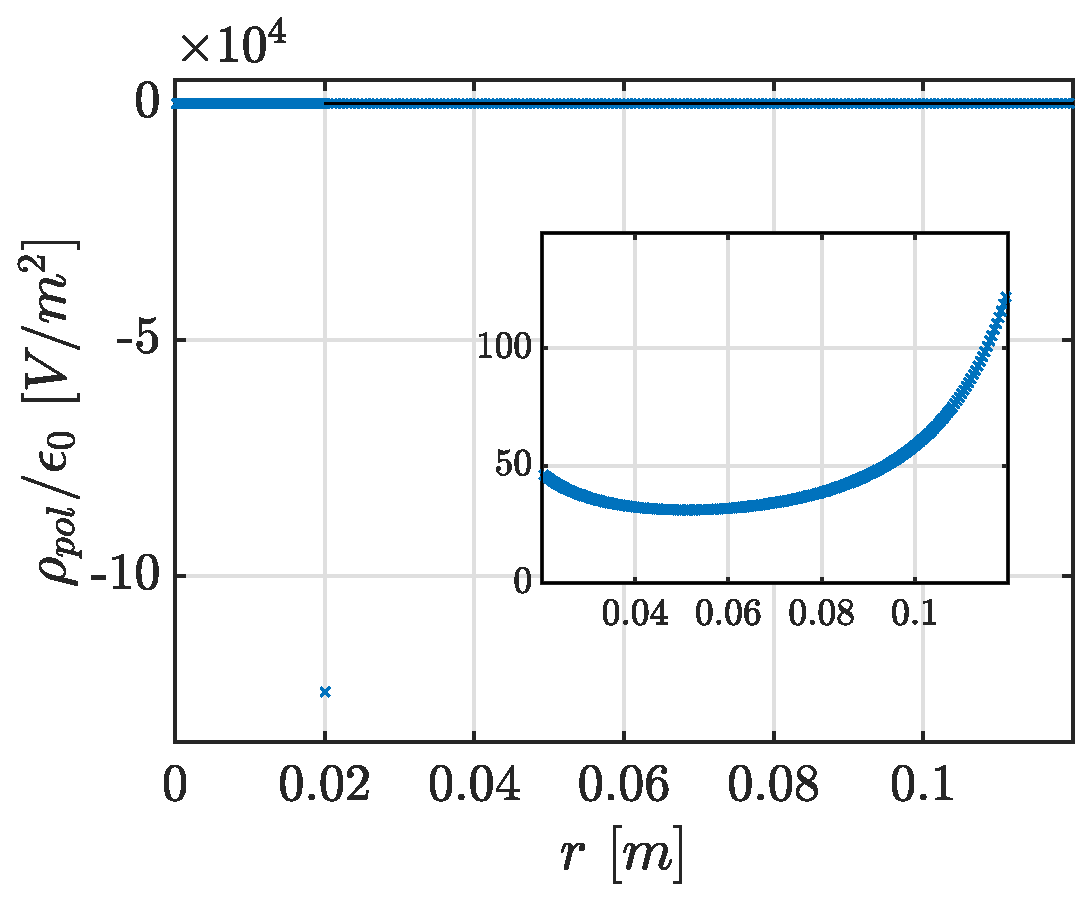
\includegraphics[width=0.5\textwidth]{graphs/exdii-rhopol.eps}
      \caption{Polarization charge density with respect to the distance $r$ to the center of the cylinder. The simulation used the settings $N_2 = 2N_1 = 200$.}
      \label{fig:rhopol}
    \end{figure}


  \subsection{Polarization charge}
  Using the result from section \ref{sec:rhopol}, it is possible to obtain the polarization charge at $r=b$.
  The polarization charge is simply the integral of $\rho_{pol}$, which is the area under the curve of figure \ref{fig:rhopol}.
  The simpliest way to obtain this area is to compute the area of the triangle surrounding $r=b$ in figure \ref{fig:rhopol}.
  Thus, the polarization charge obtained from figure \ref{fig:rhopol} is given by \SI{-3.858d-10}{\coulomb}.
  To show that the result indeed converges, a convergence study of this value is shown on figure \ref{fig:exdii-conv-polch}.
  It shows that the value of the polarization charge converges on a first order convergence.

  \begin{figure}
    \centering
    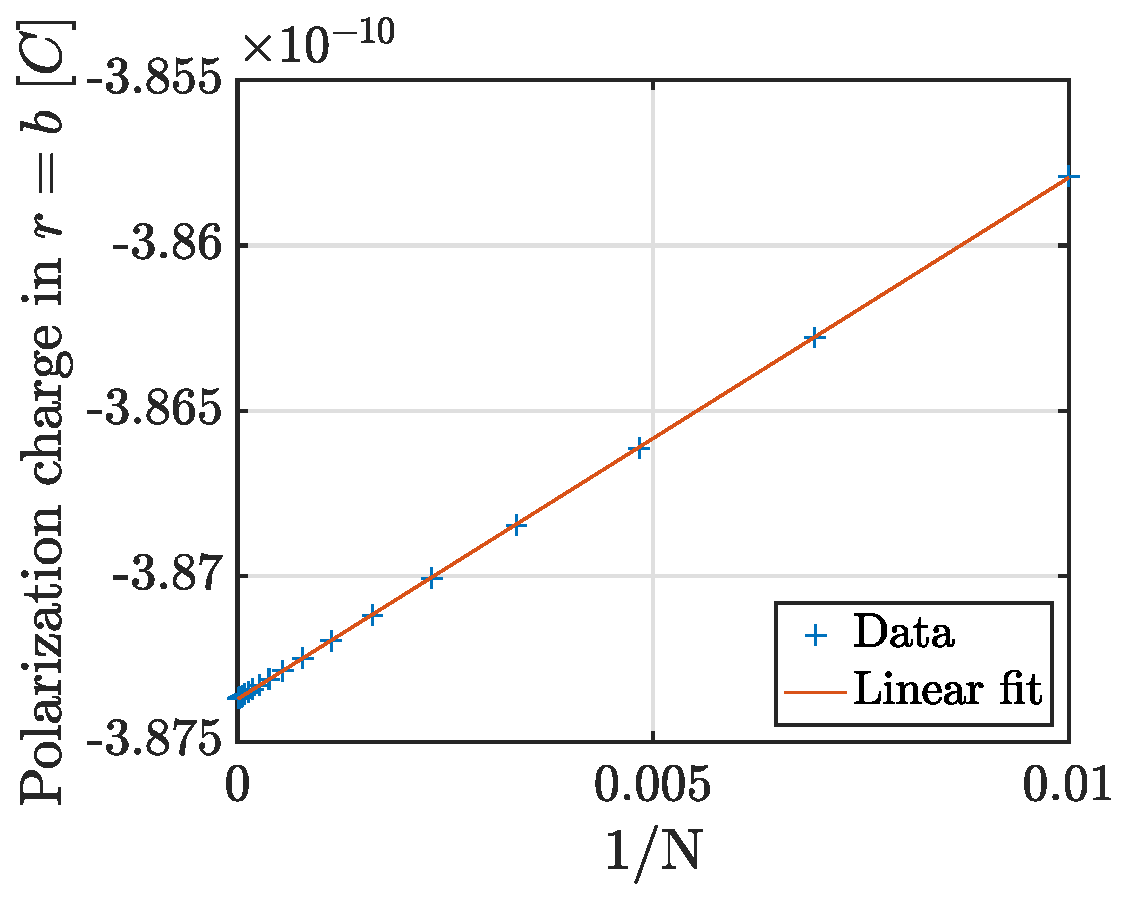
\includegraphics[width=0.5\textwidth]{graphs/exdii-conv-polch.eps}
    \caption{Convergence study of the polarization charge in $r=b$ with respect to $N$, where $N_2 = 2N_1 =2N$}
    \label{fig:exdii-conv-polch}
  \end{figure}


  \section{Supplement} %TODO : Le titre de la section pue.
    \subsection{Combination of the trapezoidal rule and the middle point rule} \label{sec:trapezoidal-middle-rule}
      Section \ref{sec:writing-A-b1} gives a method to describe the elements of the matrix $A$ and the vector $\mbf{b}$.
      These elements contained integral, which needed to be numerically approximated.
      To achieve this, the trapezoidal rule was used.
      An alternative method can be used to compute these integrals, which is a combination of the trapezoidal rule and the middle point rule.
      Let $f\bracket{x}$ be an integrable function.
      Then, the trapezoidal-middle point rule is given by equation \eqref{eq:int-trapeze-milieu}, where $p\in[0,1]$ is a parameter.
      Note that $p=1$ gives the trapezoidal rule, so the source file was updated using this new formula.

      \begin{equation}
        \int_{x_k}^{x_{k+1}}f\bracket{x}dx \approx h_k\bracket{p\frac{f\bracket{x_k} + f\bracket{x_{k+1}}}{2} + \bracket{1-p}f\bracket{\frac{x_k + x_{k+1}}{2}}}
        \label{eq:int-trapeze-milieu}
      \end{equation}

      The whole process to obtain $A$ and $\mbf{b}$ will not be described, as it is similar to what was described in section \ref{sec:writing-A-b1}.
      Only the final results will be given.
      The matrix $A$ is described by equation \eqref{eq:A-final2}%TODO: Compléter cette phrase et ajouter la matrice A.

      \begin{empheq}[box=\boxed]{align}
        \begin{split}
            A_{i,i} = &\frac{1}{h_{i-1}}\sqbracket{ \frac{p}{2}\bracket{r_{i-1}\epsilon_r\bracket{r_{i-1}} + r_i\epsilon_r\bracket{r_i}} + \bracket{1-p}\alpha_{i-1}\epsilon_r\bracket{\alpha_{i-1}}} \\
            &+ \frac{1}{h_i}\sqbracket{\frac{p}{2}\bracket{r_i\epsilon_r\bracket{r_i} + r_{i+1}\epsilon_r\bracket{r_{i+1}}} +  \bracket{1-p}\alpha_i\epsilon_r\bracket{\alpha_i}}\\
            A_{i+1, i} = A_{i, i+1} = &-\frac{1}{h_i}\sqbracket{\frac{p}{2}\bracket{r_{i+1}\epsilon_r\bracket{r_{i+1}} + r_{i}\epsilon_r\bracket{r_i}} + \bracket{1-p}\alpha_{i}\epsilon_r\bracket{\alpha_i}}
        \end{split}
        \label{eq:A-final2}
      \end{empheq}

      with $\alpha_k = \frac{r_k + r_{k+1}}{2}$.
      The vector $b_i$ is described by equation \eqref{eq:b-final2}.

      \begin{equation}
        \boxed{b_i = \frac{1}{2\epsilon_0}\sqbracket{pr_i\rho\bracket{r_i}\bracket{h_i + h_{i-1}} + \bracket{1-p}\bracket{h_{i-1}\alpha_{i-1}\rho\bracket{\alpha_{i-1}} + h_i\alpha_i\rho\bracket{\alpha_i}}}}
        \label{eq:b-final2}
      \end{equation}

      with $\alpha_k = \frac{r_k + r_{k+1}}{2}$.

      Using this new implementation, with $p=0.5$, the potential for the trivial case was plotted again in figure \ref{ephi} and compared to the analytical result. This time the plots are indistinguishable from each other, no matter how much we zoom in with MATLAB. Therefore this method for finding the elements of the matrix and the vector seems much more precise than the one that was used in previous sections.
      \begin{figure}[h]
      \centering
       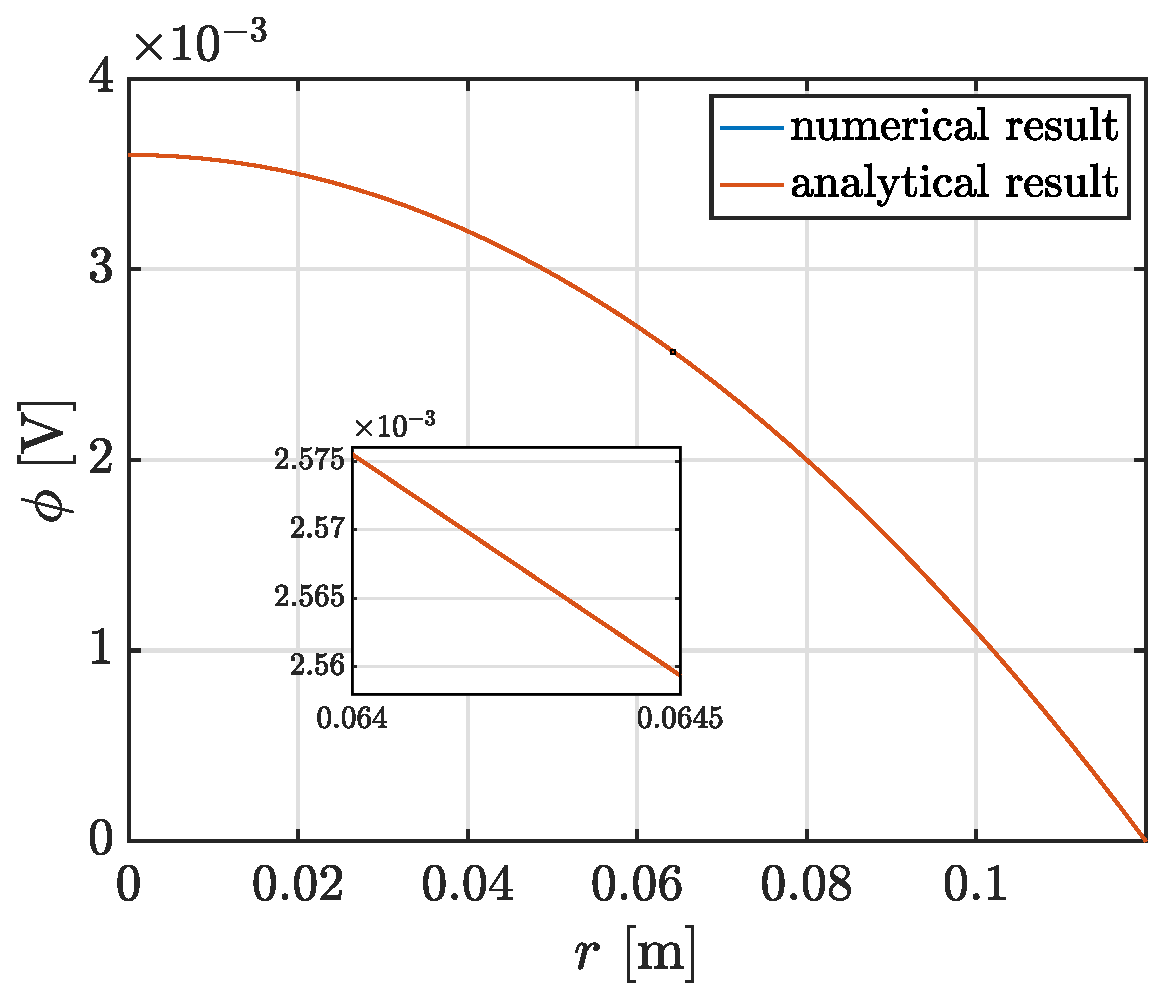
\includegraphics[width=0.5\textwidth]{graphs/e_phi.eps}
       \caption{Numerical and analytical potential in function of radius for N=20}
       \label{ephi}
      \end{figure}

  \newpage
  \begin{thebibliography}{99}
    \bibitem{wiki:dielectrics} Wikipedia contributors, "Dielectric," Wikipedia, The Free Encyclopedia, \url{https://en.wikipedia.org/w/index.php?title=Dielectric&oldid=887928781} (accessed March 22, 2019).

    \bibitem{feynman:dielectrics} Feynman, R. (n.d.). The Feynman Lectures on Physics Vol. II Ch. 10: Dielectrics. [online] Feynmanlectures.caltech.edu. Available at: \url{http://www.feynmanlectures.caltech.edu/II_10.html} [Accessed 18 Mar. 2019].
  \end{thebibliography}

\end{document}
